\subsubsection{Gleichtakt} \label{subsec:gleichtakt}
In diesem Kapitel ist Schritt für Schritt beschrieben, wie die Gleichtaktschaltung aus der Aufgabenstellung vereinfacht wird. Abbildung \ref{fig:orig_CMSchaltung} zeigt die Schaltung aus der Aufgabenstellung. Diese Schaltung ist mit den Komponenten $R_w$ und $L_r$ ergänzt worden, sodass sie symmetrisch ist(siehe Abbildung \ref{fig:CMSchaltung1}). Dies macht es möglich, dass die Schaltung zur Simulation wie folgt vereinfacht werden kann.
\begin{figure}[H]
	\centering
	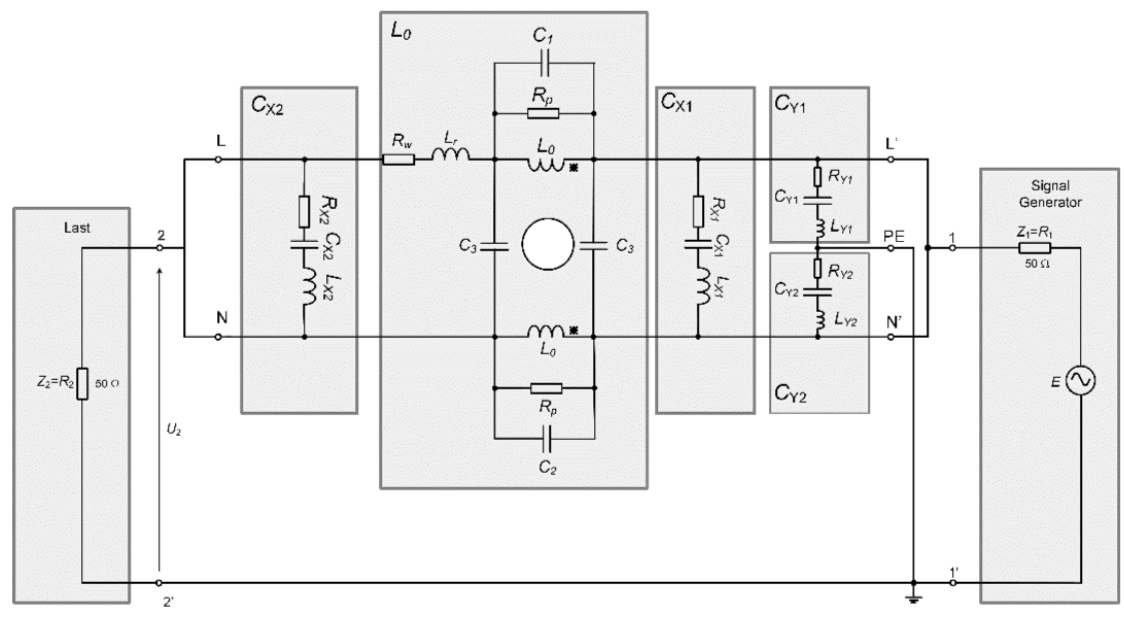
\includegraphics[width = 10cm]{CM_Aufgabenstellung.png}
	\caption{Originale Gleichtaktschaltung\cite{aufgabenstellung}}
	\label{fig:orig_CMSchaltung}
\end{figure}
\begin{figure}[H]
	\centering
	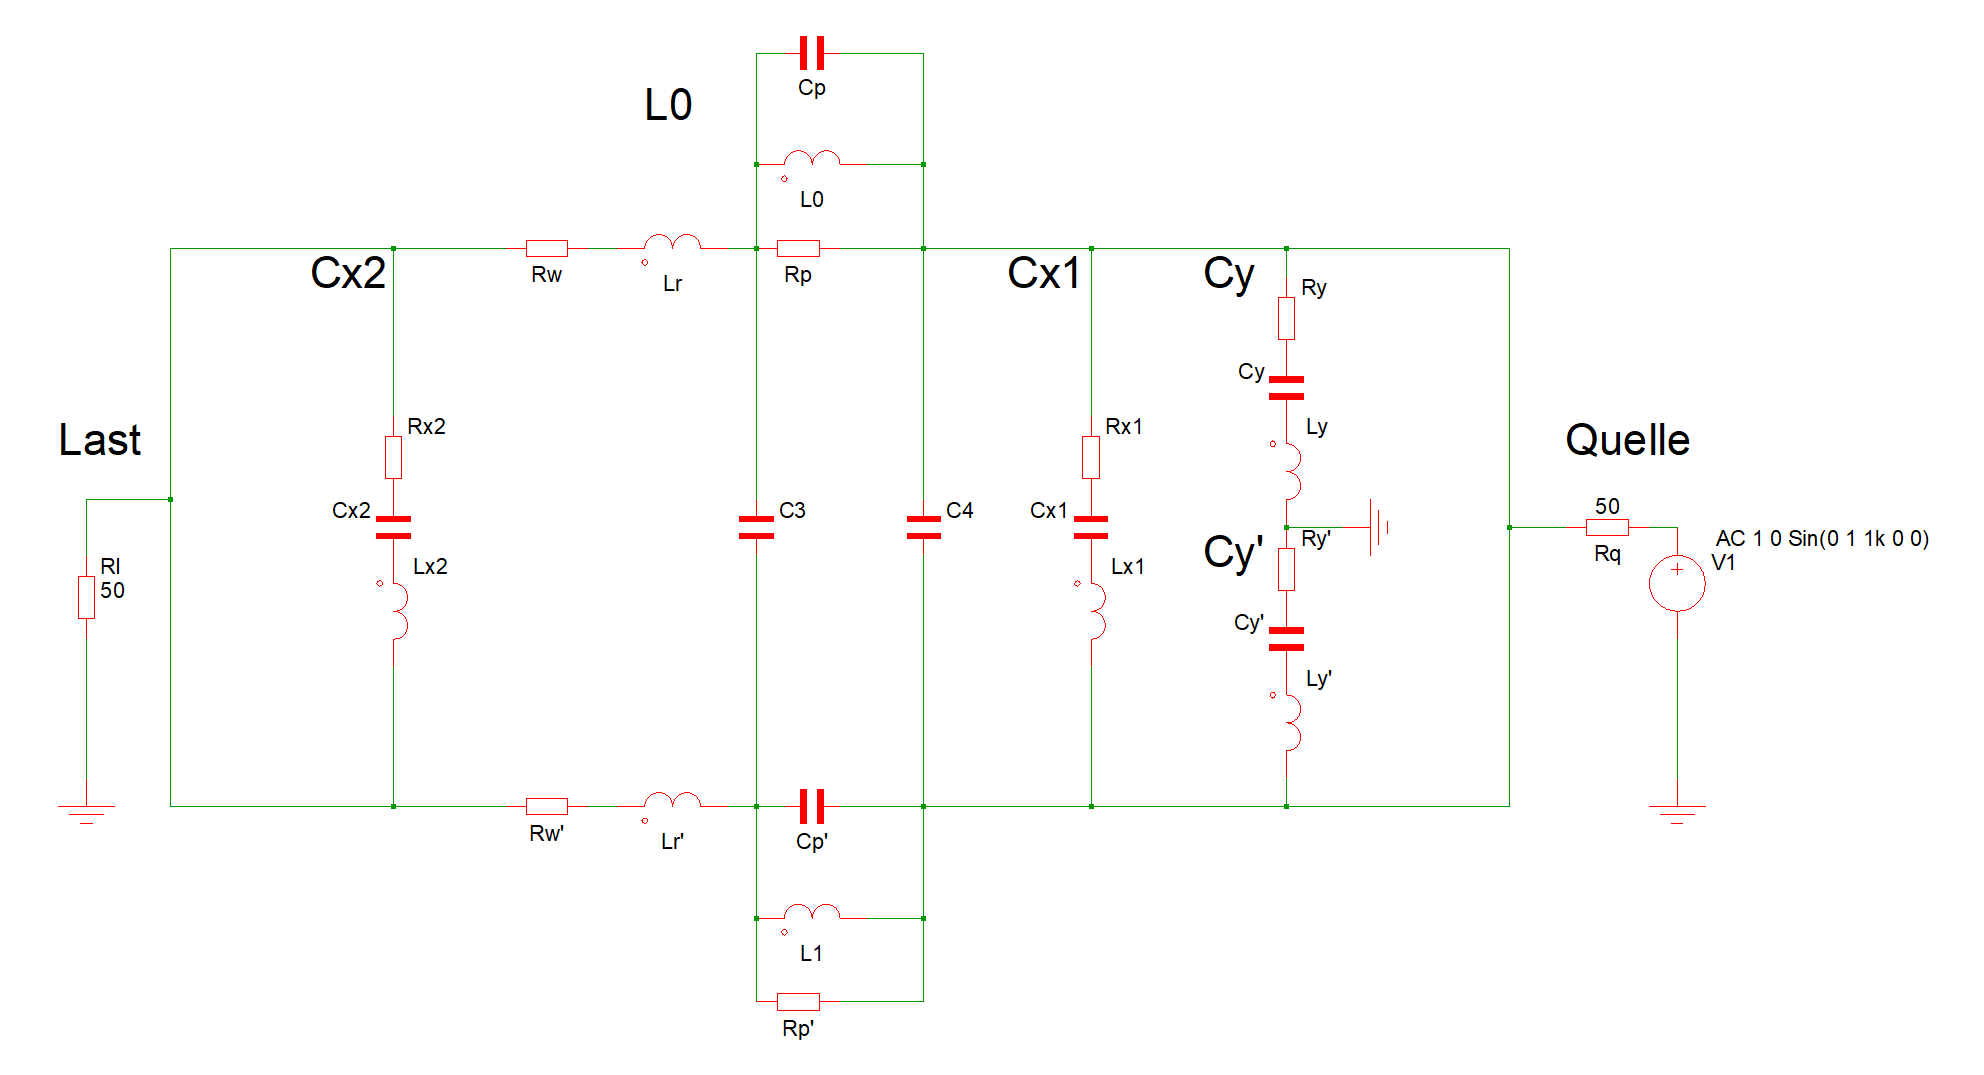
\includegraphics[width = 10cm]{EMI_CMpretty1.png}
	\caption{Ergänzte Gleichtaktschaltung}
	\label{fig:CMSchaltung1}
\end{figure}
Da der obere und untere Strang identisch sind und es keinen Potentialunterschied zwischen ihnen gibt, kann die Schaltung, wie folgt, zusammen gefasst werden (siehe Abbildung \ref{fig:CMSchaltung2}). Die Schaltung wird entlang der Symmetrie-Achse aufgetrennt. Somit fallen die Kondensatoren $C_3$, $C_4$, $C_{x1}$ und $C_{x2}$ komplett weg. Die übrigen Komponenten von $L_0$ bilden eine Parallelschaltung, welche sich durch halbieren der Widerstände und Induktivitäten und verdoppeln der Kapazitäten zusammenfassen lässt. Zusätzlich werden die beiden $C_y$ und $C'_{y}$ parallel auf das Bezugspotential geschalten. Da $C_y$ und $C'_y$ identisch sind, werden sie wie in Abbildung \ref{fig:CMSchaltung2} zusammengefasst. Diese vereinfachte Schaltung bildet die Grundlage für die Berechnungen der Software.
\begin{figure}[H]
	\centering
	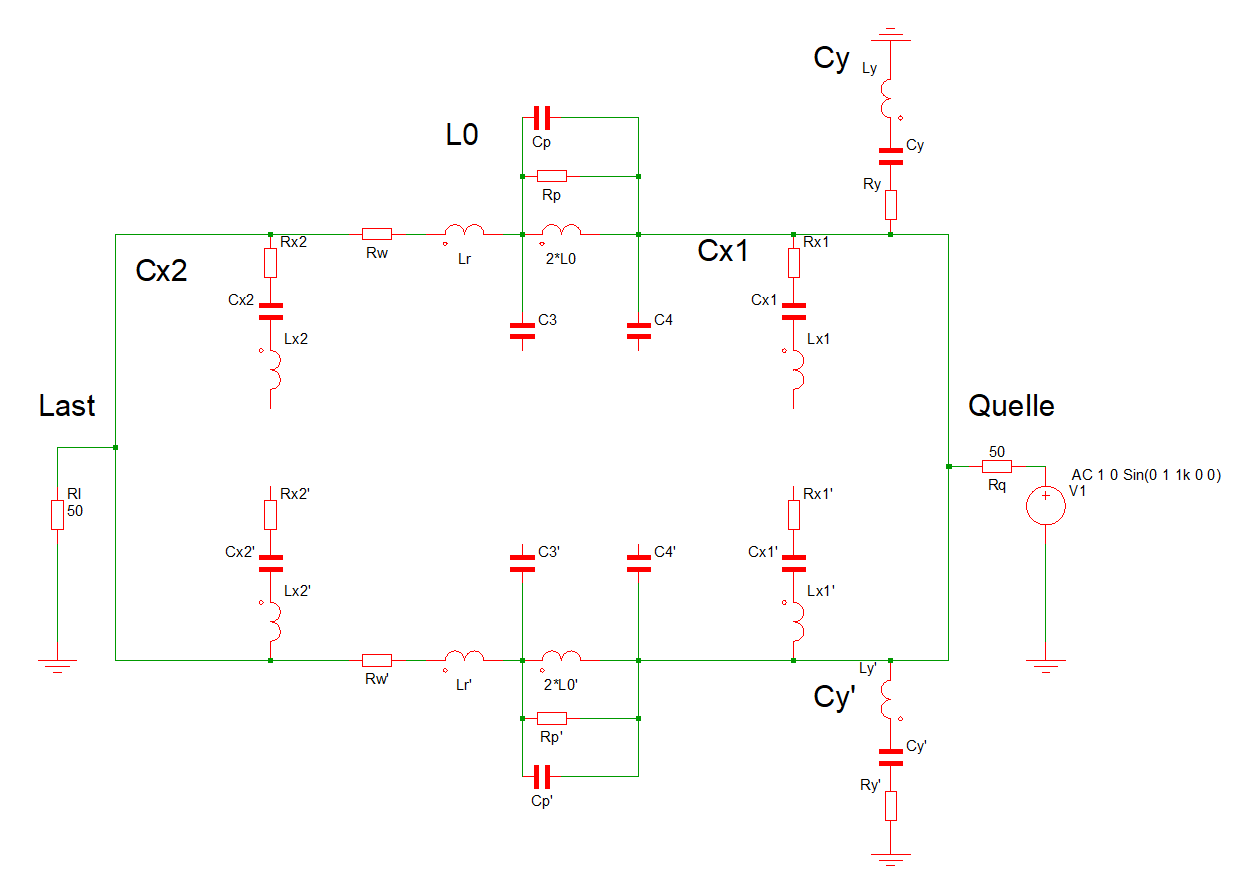
\includegraphics[width = 10cm]{EMI_CMpretty2.png}
	\caption{Vereinfachte Gleichtaktschaltung}
	\label{fig:CMSchaltung2}
\end{figure}